% Relatório de Estágio Supervisionado — Bacharelado em Sistemas de Informação / UFAC
% Estrutura baseada no modelo Word de Relatório de Estágio da UFAC.
% Conteúdo: Marcos Vinícius Moraes Costa — Biblioteca Central da UFAC.
%
% Compilação: pdfLaTeX -> BibTeX -> pdfLaTeX -> pdfLaTeX.

\documentclass[
  12pt,
  openright,
  oneside,
  a4paper,
  sumario=tradicional,
  english,
  brazilian
]{abntex2}

% O estilo UFAC e o brasão em figuras/exefig.eps foram preservados.
\usepackage{abntex2-UFAC}
\usepackage[T1]{fontenc}
\usepackage[utf8]{inputenc}
\usepackage{indentfirst}
\usepackage{graphicx}
\usepackage[outdir=./]{epstopdf} % brasão EPS do estilo UFAC
\usepackage{booktabs}
\usepackage{tikz}
\usetikzlibrary{positioning,arrows.meta} % Organograma da Biblioteca Central
\usepackage[alf,abnt-emphasize=bf]{abntex2cite}
\citeoption{AuthorYEAR}
\usepackage{mathptmx}
\renewcommand{\ABNTEXchapterfont}{\rmfamily\bfseries}

% Quadros têm numeração e lista próprias, como previsto no modelo Word.
% Comandos fornecidos pela classe memoir, utilizada pelo abnTeX2.
\newcommand{\quadroname}{Quadro}
\newcommand{\listofquadrosname}{Lista de quadros}
\newfloat[chapter]{quadro}{loq}{\quadroname}
\newlistof{listofquadros}{loq}{\listofquadrosname}
\newlistentry{quadro}{loq}{0}

\titulo{Desenvolvimento de um Sistema Web para Gestão e Controle de Uso da Sala de Informática da Biblioteca Central da Universidade Federal do Acre}
\autor{Marcos Vinícius Moraes Costa}
\local{Rio Branco}
\data{2026}
\orientador{Laura Costa Sarkis}
\instituicao{Universidade Federal do Acre}
\campus{Centro de Ciências Exatas e Tecnológicas}
\curso{Curso de Bacharelado em Sistemas de Informação}
\preambulo{Relatório de estágio supervisionado apresentado como exigência parcial para obtenção do grau de bacharel em Sistemas de Informação da Universidade Federal do Acre.}

\makeatletter
\hypersetup{
  pdftitle={\@title},
  pdfauthor={\@author},
  pdfsubject={Relatório de Estágio Supervisionado},
  colorlinks=false,
  linkcolor=black,
  citecolor=black,
  urlcolor=black,
  bookmarksdepth=4
}
\makeatother

\begin{document}
\frenchspacing
\pretextual

\imprimircapa
\imprimirfolhaderosto

% Elementos pré-textuais na ordem do modelo Word institucional.
% Substituir campos entre colchetes pelos dados definitivos.
% Elementos pré-textuais do Relatório de Estágio Supervisionado.
% Ordem e seções adaptadas do modelo Word disponibilizado pela UFAC.
% Os campos entre colchetes devem ser preenchidos antes da entrega.

% ---------------------------------------------------------
% Termo de aprovação (dados e assinaturas ainda pendentes).
% ---------------------------------------------------------
\begin{folhadeaprovacao}
  \begin{center}
    {\ABNTEXchapterfont\bfseries\large TERMO DE APROVAÇÃO\par}
    \vspace*{1.2cm}

    {\large\MakeUppercase{\imprimirautor}\par}
    \vspace*{1.2cm}

    {\ABNTEXchapterfont\bfseries\large\MakeUppercase{\imprimirtitulo}\par}
  \end{center}

  \vspace{1.3cm}
  Este relatório de estágio supervisionado foi apresentado ao Curso de
  Bacharelado em Sistemas de Informação da Universidade Federal do Acre
  (UFAC), como exigência parcial para obtenção do grau de bacharel
  em Sistemas de Informação.

  \vspace{0.6cm}
  \noindent\textbf{Data de aprovação:} [DIA/MÊS/ANO]

  \vspace{0.5cm}
  \noindent\textbf{Banca examinadora:}

  \assinatura{\textbf{Laura Costa Sarkis}\\Orientadora\\Universidade Federal do Acre}

  \assinatura{\textbf{[NOME COMPLETO DO(A) MEMBRO DA BANCA]}\\
    {[TITULAÇÃO E VÍNCULO INSTITUCIONAL]}}

  \begin{center}
    \vfill
    Rio Branco -- AC, [DIA] de [MÊS] de [ANO].
  \end{center}
\end{folhadeaprovacao}
\cleardoublepage

% ---------------------------------------------------------
% Dedicatória (opcional no texto final; espaço preservado).
% ---------------------------------------------------------
\begin{dedicatoria}
  \vspace*{\fill}
  \begin{flushright}
    \begin{minipage}{0.65\textwidth}
      \raggedleft
      \textit{[Inserir dedicatória, caso desejado.]}
    \end{minipage}
  \end{flushright}
  \vspace*{\fill}
\end{dedicatoria}
\cleardoublepage

% ---------------------------------------------------------
% Agradecimentos.
% ---------------------------------------------------------
\begin{agradecimentos}
  \noindent\textit{[Inserir os agradecimentos pessoais, acadêmicos e
  institucionais, conforme desejado.]}
\end{agradecimentos}
\cleardoublepage

% ---------------------------------------------------------
% Epígrafe (opcional no texto final; sem citação inventada).
% ---------------------------------------------------------
\begin{epigrafe}
  \vspace*{\fill}
  \begin{flushright}
    \begin{minipage}{0.65\textwidth}
      \raggedleft
      \textit{[Inserir frase ou citação escolhida.]}\\[0.6em]
      [AUTORIA DA EPÍGRAFE]
    \end{minipage}
  \end{flushright}
  \vspace*{\fill}
\end{epigrafe}
\cleardoublepage

% ---------------------------------------------------------
% Resumo e palavras-chave (a redigir após revisão dos resultados).
% ---------------------------------------------------------
\begin{resumo}
  \noindent
  \textit{[Redigir aqui um único parágrafo com a contextualização do
  estágio, o objetivo, a metodologia, as atividades desenvolvidas,
  os principais resultados comprovados e a conclusão.]}

  \vspace{\onelineskip}
  \noindent\textbf{Palavras-chave:} [Palavra-chave 1].
  [Palavra-chave 2]. [Palavra-chave 3].
\end{resumo}
\cleardoublepage

% ---------------------------------------------------------
% Abstract e keywords (tradução do resumo final).
% ---------------------------------------------------------
\begin{resumo}[Abstract]
  \begin{otherlanguage*}{english}
    \noindent
    \textit{[Write the English translation of the final Portuguese
    abstract here, including context, objectives, methods, findings,
    and conclusions.]}

    \vspace{\onelineskip}
    \noindent\textbf{Keywords:} [Keyword 1]. [Keyword 2]. [Keyword 3].
  \end{otherlanguage*}
\end{resumo}
\cleardoublepage

% ---------------------------------------------------------
% Listas automáticas, mesmo que ainda não existam ilustrações.
% Serão preenchidas pelo LaTeX conforme figuras, quadros e tabelas
% com legendas forem inseridos nos capítulos.
% ---------------------------------------------------------
\pdfbookmark[0]{\listfigurename}{lof}
\listoffigures*
\cleardoublepage

\pdfbookmark[0]{\listofquadrosname}{loq}
\listofquadros
\cleardoublepage

\pdfbookmark[0]{\listtablename}{lot}
\listoftables*
\cleardoublepage

% Siglas/abreviaturas existentes no texto. Revisar ao finalizar.
\begin{siglas}
  \item[API] Interface de Programação de Aplicações
  \item[IHC] Interação Humano-Computador
  \item[MVP] Produto Mínimo Viável
  \item[UFAC] Universidade Federal do Acre
\end{siglas}
\cleardoublepage

% Se o relatório passar a utilizar notação específica, inserir
% aqui um ambiente "simbolos" antes do sumário.


\pdfbookmark[0]{\contentsname}{toc}
\tableofcontents*
\cleardoublepage

\textual

\chapter{Introdução}\label{cap:introducao}

A Biblioteca Central Ruy Alberto Costa Lins, situada no Campus Sede da Universidade Federal do Acre (UFAC), em Rio Branco, disponibiliza computadores à comunidade acadêmica em sua Sala de Informática, também denominada Sala Virtual na documentação inicial do projeto. No início do estágio, o controle de utilização desse espaço era realizado por meio de fichas impressas de presença e de registros posteriormente reunidos para elaboração de relatórios. Embora essa rotina permitisse acompanhar os atendimentos, a consulta histórica e a consolidação das informações exigiam procedimentos manuais.

A informatização do controle envolve mais do que a transposição da ficha de papel para uma tela. Para representar o uso de computadores, é necessário relacionar as sessões dos usuários, os horários de funcionamento, as reservas futuras, o estado dos equipamentos e eventuais ocorrências. Essas informações precisam permanecer coerentes mesmo quando uma reserva é cancelada, um computador entra em manutenção ou o usuário troca de equipamento durante a sessão.

Nesse contexto, o Estágio Supervisionado teve como atividade central o desenvolvimento de um sistema web para apoiar a gestão da Sala de Informática da Biblioteca Central da UFAC. O trabalho compreendeu o levantamento das necessidades do setor, a especificação dos requisitos, a modelagem dos fluxos, a elaboração de protótipos, a implementação da aplicação, a realização de testes e a documentação do produto.

O projeto acadêmico inicial orientou as primeiras decisões. Entretanto, durante o desenvolvimento, algumas propostas foram reformuladas e o escopo foi delimitado para viabilizar um produto mínimo funcional. Este relatório distingue, portanto, o que foi planejado, o que foi implementado na versão de demonstração e o que permanece como possibilidade de evolução. Da mesma forma, a existência de funcionalidades e de testes automatizados não é tomada como evidência de implantação definitiva ou de ganho de desempenho no atendimento sem avaliação específica.

\section{Problema da pesquisa}\label{sec:problema}

O controle manual de uso reúne informações que precisam ser consultadas de maneira articulada: identificação do usuário, computador utilizado, horários de entrada e saída e histórico dos atendimentos. Quando esses dados são armazenados em folhas impressas, a busca por registros anteriores e a preparação de totalizações por período dependem de conferência e consolidação posteriores. Também se torna mais difícil obter, durante o atendimento, uma visão integrada da disponibilidade dos computadores e dos horários reservados.

Além do registro de presença, o funcionamento da sala exige a observância de regras operacionais. Uma nova reserva não pode coincidir com outra utilização válida do equipamento. Computadores indisponíveis para manutenção não devem ser oferecidos como livres. Alterações no calendário de funcionamento precisam considerar compromissos já assumidos, sem apagar as condições históricas dos atendimentos realizados. Por fim, o sistema deve apresentar informações adequadas às tarefas dos usuários da sala e da equipe responsável por sua operação.

Diante desse cenário, estabeleceu-se a seguinte questão orientadora: \emph{como um sistema web pode apoiar, de maneira organizada e acessível, o registro, o acompanhamento e a produção de informações sobre a utilização dos computadores da Sala de Informática da Biblioteca Central da UFAC?}

\section{Objetivos da pesquisa}\label{sec:objetivos}

\subsection{Objetivo geral}

Desenvolver um sistema web para organizar o registro, o acompanhamento e a geração de relatórios de utilização dos computadores da Sala de Informática da Biblioteca Central da UFAC, considerando os processos de atendimento e as regras de funcionamento do ambiente.

\subsection{Objetivos específicos}

Para alcançar o objetivo geral, o trabalho foi orientado pelos seguintes objetivos específicos:

\begin{enumerate}
    \item Analisar o processo manual e identificar os requisitos necessários à informatização do controle de uso.
    \item Modelar os atores, os dados, as regras de negócio e os principais fluxos da aplicação.
    \item Implementar a consulta de disponibilidade dos computadores e o agendamento de horários compatíveis com o funcionamento da sala.
    \item Desenvolver o registro de entrada, permanência, troca de computador e saída, preservando o histórico das sessões.
    \item Permitir o acompanhamento do estado operacional dos equipamentos e o registro de ocorrências.
    \item Construir interfaces voltadas ao Usuário da Sala, ao Monitor da Sala e ao Supervisor da Biblioteca.
    \item Produzir relatórios e indicadores derivados dos registros operacionais, com recursos de consulta e exportação.
    \item Verificar os fluxos implementados por meio de testes e documentar as decisões técnicas e os procedimentos de continuidade do sistema.
\end{enumerate}

Esses objetivos representam o recorte adotado durante a construção do produto. A fila de espera, prevista no projeto inicial, foi excluída do escopo implementado. A autenticação institucional e a interface administrativa própria também foram mantidas como evoluções futuras.

\section{Justificativa da pesquisa}\label{sec:justificativa}

A necessidade de organizar os registros de atendimento motivou o desenvolvimento do sistema. Uma base estruturada de informações sobre computadores, reservas, sessões e ocorrências permite estabelecer regras uniformes para registrar e consultar a utilização do espaço. A geração de relatórios a partir dessa mesma base pode reduzir etapas de consolidação manual e apoiar o acompanhamento por data, período e equipamento. Esses benefícios são possibilidades proporcionadas pela solução; sua magnitude dependeria de avaliação posterior no ambiente de uso.

O problema também apresenta relevância técnica. Foi necessário explicitar condições que, em um processo manual, poderiam depender da interpretação dos responsáveis pelo atendimento, como intervalos válidos para reservas, tolerâncias de entrada e saída, conflitos de utilização, alterações nos horários de funcionamento e correções de registros. O tratamento dessas condições está relacionado à especificação de requisitos verificáveis e à definição de regras consistentes, conforme discutido por \citeonline{sommerville2016} e na ISO/IEC/IEEE 29148:2018 \cite{iso29148_2018}.

As necessidades de interação variam entre os perfis. O usuário precisa localizar um computador e registrar sua utilização; o monitor acompanha as atividades em andamento; e o supervisor configura parâmetros e analisa informações consolidadas. A organização dessas tarefas em interfaces distintas encontra fundamento nas práticas de Interação Humano-Computador e de projeto centrado nas pessoas \cite{barbosaSilva2010,iso9241_210_2019}.

Do ponto de vista da formação acadêmica, o estágio possibilitou aplicar conhecimentos de Engenharia de Software, banco de dados, arquitetura de sistemas, desenvolvimento web, testes e documentação a uma demanda institucional. A preservação do código e dos artefatos técnicos também contribui para a manutenção e a eventual continuidade do produto.

\section{Metodologia}\label{sec:metodologia}

O trabalho foi de natureza aplicada e organizado em incrementos de desenvolvimento, com análise qualitativa do processo de atendimento como ponto de partida. Inicialmente, foram examinados os modelos de registro utilizados pela biblioteca e discutidas as necessidades operacionais com a supervisão. Essas informações subsidiaram a especificação de requisitos, a descrição de casos de uso, a elaboração de diagramas de atividades e a prototipação das interfaces.

Em seguida, foram definidos o modelo de domínio, as regras de operação e a arquitetura da aplicação. A implementação foi realizada por incrementos relacionados à disponibilidade de computadores, às reservas, às sessões de uso, ao calendário operacional, às ocorrências, às interfaces dos perfis e aos relatórios. O versionamento do código e a documentação das decisões técnicas acompanharam o processo.

A verificação utilizou dados fictícios, testes das regras e das interfaces de programação de aplicações (APIs), restrições de integridade no banco de dados e testes de ponta a ponta dos fluxos web. Entre os cenários previstos na documentação constam conflitos de reserva, mudanças de estado de computadores, transições de sessão, diferenciação de permissões entre perfis simulados e consistência das projeções de relatórios. Essa estratégia permitiu avaliar o comportamento implementado, sem substituir a necessidade de validação com os responsáveis pelo atendimento real.

Para redigir o relatório, foram utilizados o projeto acadêmico, as fichas de frequência e os artefatos do repositório da aplicação, incluindo requisitos, arquitetura, diagramas, decisões técnicas e registros de implementação. Resultados ainda não demonstrados, como redução mensurada do tempo de atendimento e operação contínua em produção, não foram presumidos.


\chapter{Fundamentação teórica}\label{cap:fundamentacao}

A informatização do uso de uma sala de computadores exige mais do que a implementação de formulários. É necessário compreender as atividades realizadas no ambiente, especificar regras verificáveis, preservar a consistência dos dados e apresentar operações de maneira acessível. Este capítulo reúne os conceitos que fundamentaram o desenvolvimento, aproveitando a revisão bibliográfica do projeto de estágio.

\section{Engenharia de Software}\label{sec:engenharia}

A Engenharia de Software reúne processos, métodos e práticas voltados à especificação, construção, verificação e evolução de sistemas. Conforme \citeonline{sommerville2016}, o desenvolvimento deve considerar tanto as funcionalidades necessárias quanto atributos de qualidade, manutenção e adequação ao contexto em que o produto será utilizado. Em problemas institucionais, a análise do processo existente ajuda a evitar que decisões técnicas sejam tomadas sem relação com as necessidades dos usuários.

No estágio, a elaboração de uma solução para a biblioteca começou pelo levantamento do funcionamento manual da sala e pela identificação das tarefas que precisariam ser representadas digitalmente. A definição do escopo foi importante porque o conjunto inicial de possibilidades ultrapassava o que seria desenvolvido na primeira versão funcional.

\subsection{Engenharia de requisitos}

Os requisitos funcionais descrevem os serviços e comportamentos esperados de um sistema, enquanto os não funcionais expressam propriedades e restrições relevantes para seu funcionamento. A ISO/IEC/IEEE 29148:2018 orienta os processos de Engenharia de Requisitos e a elaboração de especificações que possam ser compreendidas, avaliadas e verificadas \cite{iso29148_2018}.

No caso estudado, consultar horários, reservar um computador, registrar entrada e saída e gerar relatórios são exemplos de comportamentos funcionais. Integridade dos registros, clareza das mensagens e acessibilidade da interface exemplificam condições de qualidade. A especificação dessas necessidades deve considerar situações excepcionais, como duas tentativas concorrentes de reserva ou a indisponibilidade de um computador já associado a um atendimento.

Uma regra de negócio é uma restrição ou condição particular do domínio, associada à maneira como uma atividade deve ocorrer. Por exemplo, a consulta de disponibilidade precisa respeitar os horários de funcionamento, e a reserva deve ser rejeitada quando o intervalo solicitado entra em conflito com outra utilização válida. Regras dessa natureza não devem depender apenas da apresentação visual; elas precisam ser aplicadas pela camada responsável pelo processamento da operação.

\subsection{Modelagem e documentação}

A modelagem permite representar atores, atividades e dados antes da implementação, tornando mais explícitas as decisões sobre o funcionamento do produto. Diagramas de casos de uso apresentam objetivos e interações dos participantes com o sistema. Diagramas de atividades descrevem sequências de ações, alternativas e condições de passagem entre etapas. As descrições textuais complementam essas representações ao registrar pré-condições, validações e resultados esperados \cite{sommerville2016}.

Esses artefatos contribuem para a comunicação entre as pessoas envolvidas e para a rastreabilidade das funcionalidades. Quando uma regra é alterada, é possível revisar suas consequências nos fluxos, na implementação e nos testes correspondentes. A documentação, portanto, não se limita ao planejamento: também deve acompanhar as mudanças realizadas durante o desenvolvimento.

\section{Interação Humano-Computador}\label{sec:ihc}

A Interação Humano-Computador (IHC) considera as pessoas, suas tarefas e as condições em que utilizam sistemas interativos. \citeonline{barbosaSilva2010} discutem métodos de identificação de necessidades, elaboração de soluções e avaliação da interação. A qualidade de uma interface não depende somente de sua aparência, mas também da compreensão das informações e da facilidade de concluir tarefas.

A ISO 9241-210:2019 apresenta orientações para o projeto centrado nas pessoas, incluindo compreensão do contexto de uso, envolvimento dos usuários e avaliação iterativa das soluções \cite{iso9241_210_2019}. Para a Sala de Informática, essa abordagem é pertinente porque existem necessidades distintas: quem deseja utilizar um computador precisa consultar disponibilidade e registrar o atendimento; quem acompanha a operação precisa identificar sessões ativas e ocorrências; e quem supervisiona o ambiente precisa configurar parâmetros e consultar indicadores.

A prototipação oferece uma maneira de explorar essas necessidades antes de concluir a implementação. Representações navegáveis das telas permitem discutir a sequência de ações, a distribuição dos elementos e o tratamento de situações excepcionais. Após a implementação, verificações funcionais da navegação e avaliações de usabilidade constituem atividades complementares. A existência de uma interface responsiva ou de testes automatizados, por si só, não comprova que uma avaliação de usabilidade com participantes tenha sido realizada.

\section{Banco de dados e integridade da informação}\label{sec:banco}

Sistemas de banco de dados possibilitam o armazenamento estruturado de informações e a definição de vínculos entre entidades. A modelagem e as restrições de integridade contribuem para impedir estados inconsistentes e assegurar que consultas retornem informações compatíveis com os registros armazenados \cite{silberschatz2019}.

No controle de uso da sala, uma sessão representa a permanência de determinado usuário e pode conter diferentes alocações de computador ao longo do atendimento. Reservas representam compromissos futuros associados a intervalos de tempo, enquanto ocorrências registram problemas relacionados aos equipamentos ou às sessões. Essa separação permite preservar um histórico de trocas sem criar uma sessão distinta para cada computador utilizado.

As operações também precisam considerar concorrência. Duas solicitações simultâneas não devem resultar em reservas confirmadas para o mesmo equipamento e intervalo. Restrições no banco e operações transacionais ajudam a preservar invariantes mesmo quando diferentes solicitações chegam em momentos próximos. O tratamento de integridade deve abranger não apenas a criação de registros, mas também alterações, cancelamentos e correções auditadas.

A dimensão temporal merece atenção particular. Horários regulares de funcionamento, exceções pontuais e versões de turnos podem mudar com o tempo. Para que os relatórios históricos permaneçam compreensíveis, alterações posteriores não devem substituir indiscriminadamente as condições que vigoravam quando uma sessão foi realizada. O armazenamento de referências históricas auxilia na reprodução das totalizações.

\section{Arquitetura de aplicações web}\label{sec:arquitetura}

Uma aplicação web normalmente envolve a interação entre um navegador, componentes responsáveis pelo processamento das requisições e um mecanismo de persistência. A separação de responsabilidades favorece a organização e a manutenção do software \cite{sommerville2016}. Essa separação pode ser implementada de diferentes formas, inclusive em uma única aplicação implantável que mantenha módulos internos bem definidos.

O monólito modular reúne a execução dos componentes em uma aplicação, mas organiza responsabilidades como cadastro, configuração, operações, ocorrências e relatórios em áreas distintas do código. Trata-se de uma alternativa que pode simplificar a implantação de um sistema de escopo delimitado, preservando pontos de evolução. A adequação dessa escolha depende do contexto técnico e operacional, não constituindo uma regra geral para todos os sistemas.

Na arquitetura adotada para a aplicação da biblioteca, o backend centraliza as regras de disponibilidade, reservas e sessões. As páginas web utilizam renderização no servidor e atualizações parciais de conteúdo, enquanto uma API permite expor operações e consultas de forma estruturada. A mesma camada de serviços é reutilizada pelas interfaces, reduzindo o risco de regras diferentes para uma operação semelhante. O detalhamento das tecnologias e módulos empregados é apresentado na Seção~\ref{sec:atividades}.

\section{Acessibilidade, verificação e validação}\label{sec:qualidade}

A acessibilidade digital procura oferecer condições de acesso e interação a pessoas com diferentes necessidades. O Modelo de Acessibilidade em Governo Eletrônico (eMAG), versão 3.1, reúne recomendações pertinentes aos serviços digitais públicos \cite{emag2014}. As Web Content Accessibility Guidelines (WCAG) 2.2 apresentam critérios verificáveis relacionados, entre outros aspectos, à navegação por teclado, à identificação de controles, ao foco visível e ao contraste \cite{wcag22_2024}.

Essas referências orientam a revisão de formulários, mensagens e componentes de navegação. A utilização de recomendações de acessibilidade durante o desenvolvimento deve ser diferenciada da comprovação de conformidade integral, que exigiria uma avaliação sistemática dos critérios pertinentes e o registro dos resultados obtidos.

A verificação busca examinar se o sistema atende às especificações e regras definidas, enquanto a validação procura avaliar sua adequação às necessidades do ambiente de uso \cite{sommerville2016}. Testes de regras, APIs, banco de dados e interfaces podem identificar defeitos e regressões. Já a avaliação em contexto real requer a participação dos responsáveis pelo atendimento e a observação das atividades que o sistema deverá apoiar.

No estágio, o desenvolvimento documentado incluiu verificações automatizadas de funcionalidades e fluxos. Tais evidências sustentam afirmações sobre a implementação testada, mas não autorizam concluir, sem dados adicionais, que houve redução mensurada de tempo de atendimento, ganho de produtividade ou implantação permanente na biblioteca.

\chapter{Estágio supervisionado}\label{cap:estagio}

Este capítulo apresenta o ambiente em que o estágio foi desenvolvido, a organização dos participantes envolvidos e as atividades realizadas para a construção do sistema web de controle de utilização da Sala de Informática da Biblioteca Central da UFAC. A exposição considera o projeto acadêmico, os registros de frequência e a documentação técnica do repositório da aplicação, distinguindo funcionalidades implementadas de etapas que ainda dependem de validação institucional.

\section{Empresa}\label{sec:empresa}

O estágio foi realizado na Universidade Federal do Acre (UFAC), tendo como unidade de referência a Biblioteca Central Ruy Alberto Costa Lins, localizada no Campus Sede, em Rio Branco. O setor contemplado pelo projeto foi a Sala de Informática, também identificada como Sala Virtual na documentação inicial, espaço que disponibiliza computadores para atividades da comunidade acadêmica.

O recorte do trabalho correspondeu ao controle da utilização desses equipamentos e ao apoio às rotinas de atendimento e acompanhamento gerencial. Assim, a solução não teve como objetivo informatizar os demais serviços da biblioteca. As fichas de presença e os modelos de relatório então utilizados forneceram referências para compreender quais registros precisariam ser preservados e como poderiam ser consolidados em meio digital.

Conforme os registros do estágio, o acompanhamento no setor foi realizado por Nádia Batista Vieira, com orientação acadêmica de Laura Costa Sarkis. As fichas de frequência consultadas documentam atividades entre 27 de maio e 25 de setembro de 2026, desde o levantamento inicial e a modelagem até o desenvolvimento das interfaces, os testes e os ajustes de relatórios.

\section{Estrutura organizacional}\label{sec:estrutura}

A Biblioteca Central Ruy Alberto Costa Lins integra a estrutura da Universidade Federal do Acre. No organograma geral disponibilizado para este relatório, a Biblioteca Central aparece vinculada ao conjunto de Órgãos Suplementares, sob a estrutura da Reitoria e Vice-Reitoria. Para contextualizar o local do estágio, a Figura~\ref{fig:organograma-biblioteca} apresenta somente essa linha institucional, sem reproduzir os demais órgãos da UFAC.

\begin{figure}[htbp]
  \centering
  \resizebox{0.83\linewidth}{!}{%
    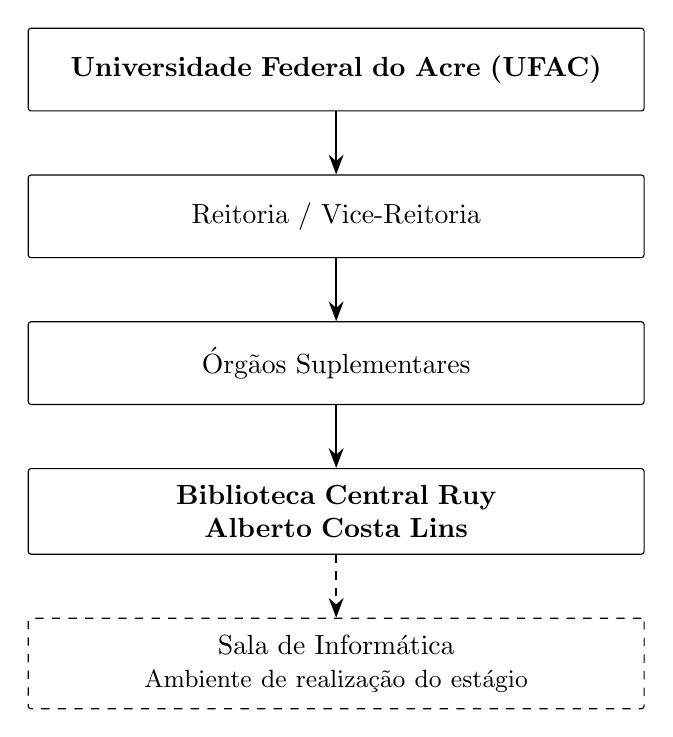
\begin{tikzpicture}[
      node distance=0.8cm,
      org/.style={
        draw,
        rectangle,
        rounded corners=1pt,
        align=center,
        text width=7.4cm,
        minimum height=1.05cm,
        inner sep=6pt,
        font=\normalsize
      },
      ambiente/.style={org,dashed},
      vinculo/.style={-{Stealth[length=2.5mm]},thick}
    ]
      \node[org] (ufac) {\textbf{Universidade Federal do Acre (UFAC)}};
      \node[org,below=of ufac] (reitoria) {Reitoria / Vice-Reitoria};
      \node[org,below=of reitoria] (orgaos) {Órgãos Suplementares};
      \node[org,below=of orgaos] (biblioteca) {\textbf{Biblioteca Central Ruy Alberto Costa Lins}};
      \node[ambiente,below=of biblioteca] (sala) {Sala de Informática\\\small Ambiente de realização do estágio};

      \draw[vinculo] (ufac) -- (reitoria);
      \draw[vinculo] (reitoria) -- (orgaos);
      \draw[vinculo] (orgaos) -- (biblioteca);
      \draw[vinculo,dashed] (biblioteca) -- (sala);
    \end{tikzpicture}%
  }
  \caption{Recorte da estrutura da UFAC com destaque para a Biblioteca Central e o ambiente do estágio}
  \label{fig:organograma-biblioteca}
  \par\smallskip
  {\footnotesize Fonte: adaptado do organograma geral da UFAC fornecido para este relatório.}
  \par\smallskip
  {\footnotesize Nota: a ligação tracejada identifica o ambiente do estágio e não pressupõe uma unidade administrativa formal independente.}
\end{figure}

O recorte indica a posição da Biblioteca Central na estrutura universitária e destaca a Sala de Informática como local específico das atividades desenvolvidas. Não foram incluídas subdivisões administrativas internas da biblioteca, pois o organograma geral consultado não apresenta esse nível de detalhamento.

A estrutura institucional não deve ser confundida com os perfis de acesso da aplicação desenvolvida. O \emph{Usuário da Sala} representa alunos, professores ou técnicos-administrativos que utilizam os computadores; o \emph{Monitor da Sala} acompanha sessões, estados dos equipamentos, ocorrências e correções; e o \emph{Supervisor da Biblioteca} possui funcionalidades adicionais de configuração, inventário e análise gerencial. O papel de \emph{Administrador do Sistema} foi previsto arquiteturalmente, mas não recebeu interface própria no MVP. Esses perfis correspondem a responsabilidades no sistema, não a cargos ou divisões confirmadas no organograma institucional.

\section{Atividades desenvolvidas}\label{sec:atividades}

As atividades ocorreram de maneira progressiva, partindo da compreensão do atendimento manual para a construção e revisão do sistema. A sequência descrita a seguir representa os principais conjuntos de trabalho e não uma reprodução diária das fichas de frequência.

\subsection{Levantamento e especificação dos requisitos}

A primeira etapa consistiu na análise do processo de controle de utilização da sala. Foram examinados os registros de presença dos usuários e os modelos de consolidação empregados pela biblioteca. A partir deles, foram identificadas as informações necessárias para registrar atendimentos e produzir relatórios, bem como as relações entre usuários, equipamentos, horários e condições de utilização.

Os requisitos foram organizados segundo as tarefas de quem utiliza a sala e de quem acompanha sua operação. Entre os fluxos prioritários estavam a consulta da disponibilidade dos computadores, a criação de reservas, a entrada e a saída do usuário, a troca de equipamento, o registro de problemas e a consulta de relatórios. Também foram consideradas restrições como evitar reservas conflitantes, impedir uso de equipamentos indisponíveis e manter informações históricas consistentes.

Durante o desenvolvimento, parte do escopo inicial foi reformulada. A fila de espera, por exemplo, deixou de integrar a versão funcional; o acesso institucional autenticado foi mantido como evolução futura. Essa delimitação permitiu concentrar a implementação nas operações centrais de controle da sala e no acompanhamento dos registros realizados.

\subsection{Modelagem e prototipação}

Com os principais requisitos definidos, foram elaborados casos de uso e diagramas de atividades referentes ao Usuário da Sala, ao Monitor da Sala e ao Supervisor da Biblioteca. Esses documentos descrevem o início das operações, as decisões intermediárias e os resultados esperados, contribuindo para explicitar regras que poderiam ser ambíguas apenas em descrições gerais.

Os diagramas de atividades contemplaram, entre outros cenários, a consulta e o agendamento de horários, o registro de entrada, a saída, a troca de computador, a comunicação de problemas e as alterações operacionais realizadas pela equipe. Também foram desenvolvidas representações visuais das telas para discutir a navegação e a apresentação das informações.

Os protótipos serviram como referência para a organização da interface, mas não foram utilizados como fonte definitiva das regras de negócio. Essas regras foram posteriormente consolidadas no backend e nos documentos de arquitetura e produto, permitindo que as interfaces apresentassem os resultados das mesmas operações sem reproduzir validações independentes.

% EVIDÊNCIA A INSERIR: selecionar um diagrama de caso de uso e um fluxo
% entre os arquivos de docs/diagrams do repositório estagio (branch dev).

\subsection{Definição da arquitetura e preparação do ambiente}

A arquitetura adotada foi a de um monólito modular desenvolvido com Python, Django e Django REST Framework, utilizando PostgreSQL para persistência. A aplicação foi organizada em módulos de responsabilidades distintas, incluindo configuração, computadores, operações, ocorrências, relatórios, auditoria e apresentação web.

Foram configurados o banco de dados, as migrações de esquema, os serviços iniciais da aplicação e o ambiente de execução com Docker Compose. A documentação técnica registra o uso de interfaces de programação de aplicações (APIs), esquemas de validação, tratamento padronizado de erros e especificação OpenAPI, além de ferramentas de formatação, verificações estáticas e integração contínua.

No modelo de domínio, foram diferenciadas as reservas, as sessões de uso e as alocações de computador. Essa decisão permite representar a permanência de uma pessoa em uma única sessão mesmo quando há troca de equipamento. Também foi distinguido o estado operacional persistido do computador, como disponível, em manutenção ou inativo, dos estados de ocupado ou reservado, calculados a partir das sessões e reservas existentes.

A organização dessas entidades exigiu restrições para evitar sobreposições de períodos e preservar a integridade das operações. Regras críticas foram implementadas nos serviços e no banco de dados, considerando que verificações feitas apenas na interface não seriam suficientes diante de solicitações simultâneas.

\subsection{Implementação das regras operacionais}

A implementação das funcionalidades centrais contemplou a consulta de computadores, a criação e o cancelamento de reservas, a entrada imediata e vinculada a uma reserva, o acompanhamento da sessão ativa, a troca de equipamento e o registro de saída. Também foram desenvolvidos mecanismos de registro e tratamento de ocorrências, alteração de estados operacionais e correção auditada de históricos.

O sistema trabalha com um calendário operacional que estabelece as janelas de funcionamento da sala e admite horários regulares, períodos temporários e exceções pontuais. As reservas são organizadas em intervalos consecutivos de 15 minutos, com validação das condições de disponibilidade. Na versão implementada, a consulta é limitada ao dia atual e ao seguinte: o uso imediato ocorre no dia corrente, e as reservas podem ser feitas para horários futuros de hoje ou de amanhã.

Foram definidas tolerâncias operacionais para entrada vinculada a reserva e para encerramento de sessão, bem como mecanismos de reconciliação dos prazos vencidos. Essas rotinas evitam que reservas ou sessões permaneçam apresentadas como válidas após o esgotamento de prazos relevantes, independentemente de o usuário atualizar manualmente a página.

Outro conjunto de regras trata da indisponibilidade de computadores. Quando um equipamento passa à condição de manutenção ou inatividade, a aplicação considera os impactos sobre as sessões e reservas relacionadas, realizando transferências ou cancelamentos conforme a possibilidade de utilização de outro computador. O procedimento foi projetado para manter coerência entre registros operacionais e histórico.

\subsection{Desenvolvimento das interfaces}

A camada de apresentação foi construída com Django Templates, HTMX, Alpine.js e Tailwind CSS, seguindo uma estratégia de interface responsiva e atualizações parciais orientadas pelo servidor. A aplicação permite selecionar perfis simulados, mas essa seleção não representa autenticação institucional real. As regras efetivas continuam concentradas nos serviços do backend.

A área do Usuário da Sala oferece consulta da situação da sala, visualização de computadores e horários, reservas, início e encerramento de sessões, troca de equipamento e comunicação de problemas. A área do Monitor da Sala apresenta informações operacionais, como sessões ativas, computadores, ocorrências e histórico, permitindo ações de acompanhamento e correção conforme as regras definidas.

O Supervisor da Biblioteca dispõe das funcionalidades operacionais e de recursos adicionais para cadastrar computadores, configurar turnos, administrar o calendário e suas exceções, publicar avisos, ajustar políticas e analisar relatórios. As telas foram organizadas com atenção à navegação em computadores e dispositivos móveis, incluindo revisão de mensagens, comportamento dos formulários e estados visuais dos componentes.

Foram realizados ajustes de acessibilidade relacionados à navegação por teclado, ao foco visível e ao contraste. Esses ajustes demonstram preocupação com a interação, mas não devem ser interpretados como certificação de conformidade integral com os critérios de acessibilidade.

% EVIDÊNCIAS A INSERIR: capturas reais das telas dos três perfis.
% As figuras devem ser produzidas a partir da aplicação, não do template anterior.

\subsection{Relatórios e indicadores de utilização}

A produção de relatórios foi uma das necessidades identificadas no processo manual de acompanhamento da sala. O sistema implementou visões diária, mensal e anual, além de indicadores de utilização, geradas a partir dos registros operacionais. Esses resultados são calculados com base em sessões, alocações, reservas, calendário, turnos e informações relacionadas.

A abordagem evita o lançamento de totais desconectados dos eventos que lhes deram origem. Os relatórios permitem diferentes recortes e agrupamentos, incluindo período, turno e computador, e podem ser exportados nos formatos CSV, XLSX e PDF. A documentação do sistema registra verificações de coerência entre os dados apresentados nas telas, as respostas das APIs e os arquivos gerados.

A versão documentada não possui relatório semanal específico, embora essa possibilidade estivesse mencionada no planejamento inicial. Também não há evidências de que os relatórios tenham sido utilizados regularmente pela biblioteca em produção. Por esse motivo, os resultados aqui descritos correspondem às funcionalidades construídas e testadas no ambiente de desenvolvimento.

\subsection{Testes, correções e documentação}

O desenvolvimento foi acompanhado por testes de regras de negócio, APIs, restrições de banco de dados e fluxos de interface. A documentação registra casos envolvendo conflitos de reservas, indisponibilidade de computadores, transições de sessões, alterações de calendário, histórico de alocações e acesso aos relatórios conforme os perfis simulados.

Também foram estruturados testes de ponta a ponta, executados sobre a aplicação Django com banco PostgreSQL de teste e cenários de dados controlados. A utilização de dados fictícios e relógio controlado auxilia na repetição de cenários dependentes de horários, enquanto a verificação das respostas do backend permite avaliar comportamentos que não são observáveis apenas pela interface.

As correções incluíram ajustes de validação, refinamento de formulários, consistência das consultas, apresentação de estados e desempenho de operações específicas. O código foi mantido em repositório Git e acompanhado por documentos de produto, arquitetura, decisões arquiteturais, diagramas e orientações de configuração. Esses artefatos fornecem uma referência para manutenção e continuidade do trabalho.

\section{Resultados obtidos}\label{sec:resultados}

O principal resultado técnico do estágio foi a construção de uma versão funcional de demonstração de um sistema web para apoiar o controle de utilização da Sala de Informática. A documentação da aplicação registra a implementação de reservas, sessões de uso, troca de computadores, saída, ocorrências, controle de equipamentos, calendário operacional e relatórios gerenciais.

As interfaces dos três perfis centrais foram implementadas: o Usuário da Sala pode executar os principais fluxos de utilização; o Monitor da Sala dispõe de recursos para acompanhar e corrigir a operação; e o Supervisor da Biblioteca acessa configurações e informações consolidadas. O sistema também dispõe de APIs e de mecanismos de integridade para preservar a coerência dos registros em operações críticas.

No conjunto de relatórios, a implementação inclui visões diária, mensal e anual, indicadores e exportações em CSV, XLSX e PDF. Os dados são obtidos dos registros operacionais, em vez de totais preenchidos manualmente. Essa característica oferece uma base técnica para reproduzir análises de utilização e investigar a origem dos resultados apresentados.

A verificação foi apoiada por testes automatizados e cenários fictícios que abrangem serviços, banco de dados, APIs e interfaces. A documentação técnica descreve essas coberturas e os procedimentos de execução. Entretanto, este relatório ainda não apresenta métricas consolidadas de aprovação dos testes, medições de desempenho em ambiente real nem resultados de uma avaliação de usabilidade com participantes da biblioteca. Esses elementos devem ser acrescentados somente após coleta e verificação das evidências correspondentes.

Permanecem fora do produto implementado a fila de espera, a autenticação institucional real, a interface funcional própria do Administrador e o relatório semanal específico. Essa delimitação deve ser considerada na comparação entre o projeto inicialmente proposto e a versão entregue para demonstração.

Dessa forma, os resultados demonstram a materialização técnica de parte substancial do escopo planejado e a disponibilidade de uma base documentada para continuidade e validação. Não se afirma, contudo, que o sistema já substituiu o controle manual utilizado pela biblioteca ou que produziu ganhos quantitativos de produtividade, pois tais conclusões exigem acompanhamento no ambiente institucional.

% PENDÊNCIAS PARA A VERSÃO FINAL:
% 1. Inserir capturas de tela verificadas dos três perfis e dos relatórios.
% 2. Inserir diagramas selecionados e respectivas fontes.
% 3. Confirmar o organograma da Biblioteca com a supervisão.
% 4. Apresentar evidências verificáveis de testes/avaliações, se disponíveis.
% 5. Diferenciar claramente demonstração, validação local e implantação real.


% Capítulo 4: considerações finais e recomendações, a redigir após revisão
% das evidências e da validação com os responsáveis pelo estágio.

\postextual
\bibliography{referencias_estagio}

\end{document}
